\section{Svolgimento dello stage}
	\subsection{}
		\begin{frame}{Metodologia di lavoro}
			\begin{minipage}{0.49\textwidth}
				\centering
				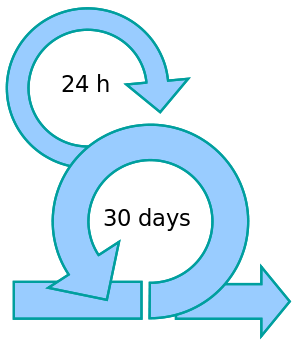
\includegraphics[width=0.5\textwidth]{capitolo_3/immagini/scrum.png}					
			\end{minipage}
			\begin{minipage}{0.49\textwidth}
				\centering
				
\includegraphics[width=0.7\textwidth]{capitolo_3/immagini/meeting.png}
			\end{minipage}\par
			\begin{minipage}{0.49\textwidth}
				\centering
				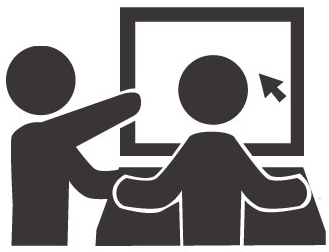
\includegraphics[width=0.5\textwidth]{capitolo_3/immagini/pair_programming.png}					
			\end{minipage}
			\begin{minipage}{0.49\textwidth}
				\centering
				
\includegraphics[width=0.7\textwidth]{capitolo_3/immagini/pianificazione.png}
			\end{minipage}			
		\end{frame}
	\subsection{Sviluppo di PastBook Mobile SDK}
		\begin{frame}{Autenticazione a Facebook e Instagram}
			\fontsize{8pt}{7}\selectfont
			\begin{figure}[H]
	\centering
	\begin{tikzpicture}
		\draw[fill=azzurro] (0,0.07\textwidth) rectangle ++(0.20\textwidth,0.12\textwidth);
		\draw (0,0.07\textwidth) rectangle ++(0.20\textwidth,0.12\textwidth)
		node[pos=.5, text width=0.18\textwidth, align=center] {Controllo stato autenticazione};
		\draw[->] (0.21\textwidth,0.13\textwidth) -- (0.25\textwidth,0.13\textwidth);
		\draw (0.1\textwidth,0.20\textwidth) -- (0.1\textwidth,0.27\textwidth);
		\draw (0.1\textwidth,0.27\textwidth) -- (0.61\textwidth,0.27\textwidth);
		\draw[->] (0.61\textwidth,0.27\textwidth) -- (0.61\textwidth,0.20\textwidth);
		\draw[fill=azzurro] (0.26\textwidth,0.07\textwidth) rectangle ++(0.20\textwidth,0.12\textwidth);
		\draw (0.26\textwidth,0.07\textwidth) rectangle ++(0.20\textwidth,0.12\textwidth)
		node[pos=.5, text width=0.18\textwidth, align=center] {Autenticazione};
		\draw[->] (0.47\textwidth,0.13\textwidth) -- (0.51\textwidth,0.13\textwidth);
		\draw[fill=azzurro] (0.52\textwidth,0.07\textwidth) rectangle ++(0.20\textwidth,0.12\textwidth);
		\draw (0.52\textwidth,0.07\textwidth) rectangle ++(0.20\textwidth,0.12\textwidth)
		node[pos=.5, text width=0.18\textwidth, align=center] {Controllo stato autorizzazione};
		\draw[->] (0.73\textwidth,0.13\textwidth) -- (0.77\textwidth,0.13\textwidth);
		\draw[fill=azzurro] (0.78\textwidth,0.07\textwidth) rectangle ++(0.20\textwidth,0.12\textwidth);
		\draw (0.78\textwidth,0.07\textwidth) rectangle ++(0.20\textwidth,0.12\textwidth)
		node[pos=.5, text width=0.18\textwidth, align=center] {Autorizzazione};
		
		\draw[dashed] (0.49\textwidth,0.2\textwidth) -- (0.49\textwidth,0.13\textwidth);
		\draw (0.41\textwidth,0.2\textwidth) rectangle ++(0.16\textwidth,0.06\textwidth)
		node[pos=.5, text width=0.16\textwidth, align=center] {Credenziali corrette};
		
		\draw (0.39\textwidth,0.06\textwidth) -- (0.39\textwidth,0);
		\draw (0.39\textwidth,0) -- (0.43\textwidth,0);
		\draw[->] (0.43\textwidth,0) -- (0.43\textwidth,0.06\textwidth);
		\draw[dashed] (0.43\textwidth,0.03\textwidth) -- (0.47\textwidth,0.03\textwidth);
		\draw (0.47\textwidth,0) rectangle ++(0.16\textwidth,0.06\textwidth)
		node[pos=.5, text width=0.16\textwidth, align=center] {Credenziali errate};
		
		\draw (0.36\textwidth,0.06\textwidth) -- (0.36\textwidth,-0.07\textwidth);
		\draw[->] (0.36\textwidth,-0.07\textwidth) -- (0.38\textwidth,-0.07\textwidth);
		\draw (0.88\textwidth,0.06\textwidth) -- (0.88\textwidth,-0.07\textwidth);
		\draw[->] (0.88\textwidth,-0.07\textwidth) -- (0.6\textwidth,-0.07\textwidth);
		\draw[fill=azzurro] (0.39\textwidth,-0.13\textwidth) rectangle ++(0.20\textwidth,0.12\textwidth);
		\draw (0.39\textwidth,-0.13\textwidth) rectangle ++(0.20\textwidth,0.12\textwidth)
		node[pos=.5, text width=0.18\textwidth, align=center] {Errore};
		
		\draw[->] (0.63\textwidth,0.2\textwidth) -- (0.63\textwidth,0.32\textwidth);
		\draw (0.88\textwidth,0.2\textwidth) -- (0.88\textwidth,0.35\textwidth);
		\draw[->] (0.88\textwidth,0.35\textwidth) -- (0.73\textwidth,0.35\textwidth);
		
		\draw[dashed] (0.83\textwidth,0.39\textwidth) -- (0.83\textwidth,0.35\textwidth);
		\draw (0.75\textwidth,0.39\textwidth) rectangle ++(0.16\textwidth,0.06\textwidth)
		node[pos=.5, text width=0.16\textwidth, align=center] {Concessi uno o più permessi};
		
		\draw[fill=azzurro] (0.52\textwidth,0.33\textwidth) rectangle ++(0.20\textwidth,0.12\textwidth);
		\draw (0.52\textwidth,0.33\textwidth) rectangle ++(0.20\textwidth,0.12\textwidth)
		node[pos=.5, text width=0.18\textwidth, align=center] {Ottenimento token};
		
		\draw[dashed] (0.36\textwidth,-0.04\textwidth) -- (0.31\textwidth,-0.04\textwidth);
		\draw (0.15\textwidth,-0.11\textwidth) rectangle ++(0.16\textwidth,0.1\textwidth)
		node[pos=.5, text width=0.16\textwidth, align=center] {Mancato inserimento credenziali};
		
		\draw[dashed] (0.75\textwidth,0.2\textwidth) -- (0.75\textwidth,0.13\textwidth);
		\draw (0.67\textwidth,0.2\textwidth) rectangle ++(0.16\textwidth,0.1\textwidth)
		node[pos=.5, text width=0.16\textwidth, align=center] {Alcuni permessi mancanti};
		
		\draw[dashed] (0.49\textwidth,0.3\textwidth) -- (0.63\textwidth,0.3\textwidth);
		\draw (0.33\textwidth,0.28\textwidth) rectangle ++(0.16\textwidth,0.1\textwidth)
		node[pos=.5, text width=0.15\textwidth, align=center] {Applicazione già autorizzata};
		
		\draw[dashed] (0.75\textwidth,-0.04\textwidth) -- (0.75\textwidth,-0.07\textwidth);
		\draw (0.67\textwidth,-0.04\textwidth) rectangle ++(0.16\textwidth,0.1\textwidth)
		node[pos=.5, text width=0.16\textwidth, align=center] {Nessun permesso concesso};
		
		\draw[dashed] (0.23\textwidth,0.13\textwidth) -- (0.23\textwidth,0.06\textwidth);
		\draw (0.15\textwidth,0) rectangle ++(0.16\textwidth,0.06\textwidth)
		node[pos=.5, text width=0.16\textwidth, align=center] {Utente non autenticato};
		
		\draw[dashed] (0.2\textwidth,0.27\textwidth) -- (0.2\textwidth,0.32\textwidth);
		\draw (0.12\textwidth,0.32\textwidth) rectangle ++(0.16\textwidth,0.06\textwidth)
		node[pos=.5, text width=0.16\textwidth, align=center] {Utente autenticato};
	\end{tikzpicture}
	\caption{Ottenimento token da Facebook o Instagram per l'autorizzazione dell'applicazione}
\end{figure}

		\end{frame}
	\subsection{Sviluppo di PastBook Mobile SDK}
		\begin{frame}{\emph{Launcher}}
			\begin{minipage}{0.97\textwidth}
				\begin{block}{Problema dell'approccio di PastBook}
					Il codice deve essere modificato quando l'algoritmo di creazione di un
					\emph{Photo Book} cambia
				\end{block}
			\end{minipage}\par
			\begin{minipage}{0.29\textwidth}
				
\includegraphics[width=0.9\textwidth]{capitolo_3/immagini/modifica_algoritmo.png}
			\end{minipage}
			\begin{minipage}{0.67\textwidth}
				\begin{block}{Soluzione proposta}
					\begin{itemize}
						\item Algoritmo modificabile da remoto
						\item Utilizzo di qualsiasi \emph{Service}
						\item Funzioni \emph{play}/\emph{pause}
						\item Uso dei risultati intermedi
					\end{itemize}
				\end{block}
			\end{minipage}
		\end{frame}
	\subsection{Sviluppo di PastBook Mobile SDK}
		\begin{frame}{Funzionamento del \emph{Launcher}}
			\fontsize{8pt}{7}\selectfont
			\begin{block}{Tipologie di \emph{Service} aziendali}
				\begin{description}
					\item[\emph{Provider}] Ottiene un insieme di foto dell'utente
					\item[\emph{Filter}] Modifica un insieme di foto
					\item[\emph{Maker}] Svolge un'azione complessa usando un insieme di foto	
				\end{description}
			\end{block}
			\begin{figure}[H]
	\centering
	\begin{tikzpicture}
		\draw[dotted] (0,0.14\textwidth) -- (0.97\textwidth,0.14\textwidth);
		\draw[dotted] (0,-0.01\textwidth) -- (0,0.14\textwidth);
	
		\draw[fill=azzurro] (0.01\textwidth,0.01\textwidth) rectangle ++(0.18\textwidth,0.08\textwidth);
		\draw (0.01\textwidth,0.01\textwidth) rectangle ++(0.18\textwidth,0.08\textwidth)
		node[pos=.5, text width=0.17\textwidth, align=center] {Get Configuration};
		
		\draw[->] (0.20\textwidth,0.05\textwidth) -- (0.24\textwidth,0.05\textwidth);
		
		\draw[fill=azzurro] (0.25\textwidth,0.01\textwidth) rectangle ++(0.18\textwidth,0.08\textwidth);
		\draw (0.25\textwidth,0.01\textwidth) rectangle ++(0.18\textwidth,0.08\textwidth)
		node[pos=.5, text width=0.17\textwidth, align=center] {Call Provider};
		
		\draw (0.32\textwidth,0.10\textwidth) -- (0.32\textwidth,0.13\textwidth);
		\draw (0.32\textwidth,0.13\textwidth) -- (0.36\textwidth,0.13\textwidth);
		\draw[->] (0.36\textwidth,0.13\textwidth) -- (0.36\textwidth,0.10\textwidth);
		
		\draw[->, dashed] (0.34\textwidth,0.13\textwidth) -- (0.34\textwidth,0.18\textwidth);
		\draw[dashed] (0.46\textwidth,0.05\textwidth) -- (0.46\textwidth,0.15\textwidth);
		\draw[dashed] (0.34\textwidth,0.15\textwidth) -- (0.46\textwidth,0.15\textwidth);
		
		\draw[->] (0.44\textwidth,0.05\textwidth) -- (0.48\textwidth,0.05\textwidth);
		
		\draw[fill=azzurro] (0.49\textwidth,0.01\textwidth) rectangle ++(0.18\textwidth,0.08\textwidth);
		\draw (0.49\textwidth,0.01\textwidth) rectangle ++(0.18\textwidth,0.08\textwidth)
		node[pos=.5, text width=0.17\textwidth, align=center] {Call Filter};
		
		\draw (0.56\textwidth,0.10\textwidth) -- (0.56\textwidth,0.13\textwidth);
		\draw (0.56\textwidth,0.13\textwidth) -- (0.60\textwidth,0.13\textwidth);
		\draw[->] (0.60\textwidth,0.13\textwidth) -- (0.60\textwidth,0.10\textwidth);
		
		\draw[->, dashed] (0.58\textwidth,0.13\textwidth) -- (0.58\textwidth,0.18\textwidth);
		\draw[dashed] (0.70\textwidth,0.05\textwidth) -- (0.70\textwidth,0.15\textwidth);
		\draw[dashed] (0.58\textwidth,0.15\textwidth) -- (0.70\textwidth,0.15\textwidth);
		
		\draw[->] (0.68\textwidth,0.05\textwidth) -- (0.72\textwidth,0.05\textwidth);
		
		\draw[fill=azzurro] (0.73\textwidth,0.01\textwidth) rectangle ++(0.18\textwidth,0.08\textwidth);
		\draw (0.73\textwidth,0.01\textwidth) rectangle ++(0.18\textwidth,0.08\textwidth)
		node[pos=.5, text width=0.17\textwidth, align=center] {Call Maker};
		
		\draw (0.80\textwidth,0.10\textwidth) -- (0.80\textwidth,0.13\textwidth);
		\draw (0.80\textwidth,0.13\textwidth) -- (0.84\textwidth,0.13\textwidth);
		\draw[->] (0.84\textwidth,0.13\textwidth) -- (0.84\textwidth,0.10\textwidth);
		
		\draw[->, dashed] (0.82\textwidth,0.13\textwidth) -- (0.82\textwidth,0.18\textwidth);
		\draw[dashed] (0.94\textwidth,0.05\textwidth) -- (0.94\textwidth,0.15\textwidth);
		\draw[dashed] (0.82\textwidth,0.15\textwidth) -- (0.94\textwidth,0.15\textwidth);
		
		
		\draw[dotted] (0.97\textwidth,0.14\textwidth) -- (0.97\textwidth,-0.01\textwidth);
		\draw[dotted] (0,-0.01\textwidth) -- (0.97\textwidth,-0.01\textwidth);
		
		
		\draw (0.25\textwidth,0.19\textwidth) rectangle ++(0.18\textwidth,0.06\textwidth)
		node[pos=.5, text width=0.17\textwidth, align=center] {Provider callback};
		
		\draw (0.49\textwidth,0.19\textwidth) rectangle ++(0.18\textwidth,0.06\textwidth)
		node[pos=.5, text width=0.16\textwidth, align=center] {Filter callback};
		
		\draw (0.73\textwidth,0.19\textwidth) rectangle ++(0.18\textwidth,0.06\textwidth)
		node[pos=.5, text width=0.17\textwidth, align=center] {Maker callback};
		
		
		\draw (0.01\textwidth,-0.10\textwidth) rectangle ++(0.18\textwidth,0.06\textwidth)
		node[pos=.5, text width=0.17\textwidth, align=center] {Start Launcher};
		
		\draw[->] (0.10\textwidth,-0.03\textwidth) -- (0.10\textwidth,0);
		
		
		\draw (0.73\textwidth,-0.10\textwidth) rectangle ++(0.18\textwidth,0.06\textwidth)
		node[pos=.5, text width=0.17\textwidth, align=center] {Photo Book};
		
		\draw (0.92\textwidth,0.05\textwidth) -- (0.96\textwidth,0.05\textwidth);
		\draw (0.96\textwidth,0.05\textwidth) -- (0.96\textwidth,-0.07\textwidth);
		\draw[->] (0.96\textwidth,-0.07\textwidth) -- (0.92\textwidth,-0.07\textwidth);
	\end{tikzpicture}
\end{figure}

		\end{frame}
	\subsection{Sviluppo di My Year Photo Book}
		\begin{frame}{Analisi dei requisiti}
			\begin{figure}[H]
				\centering
				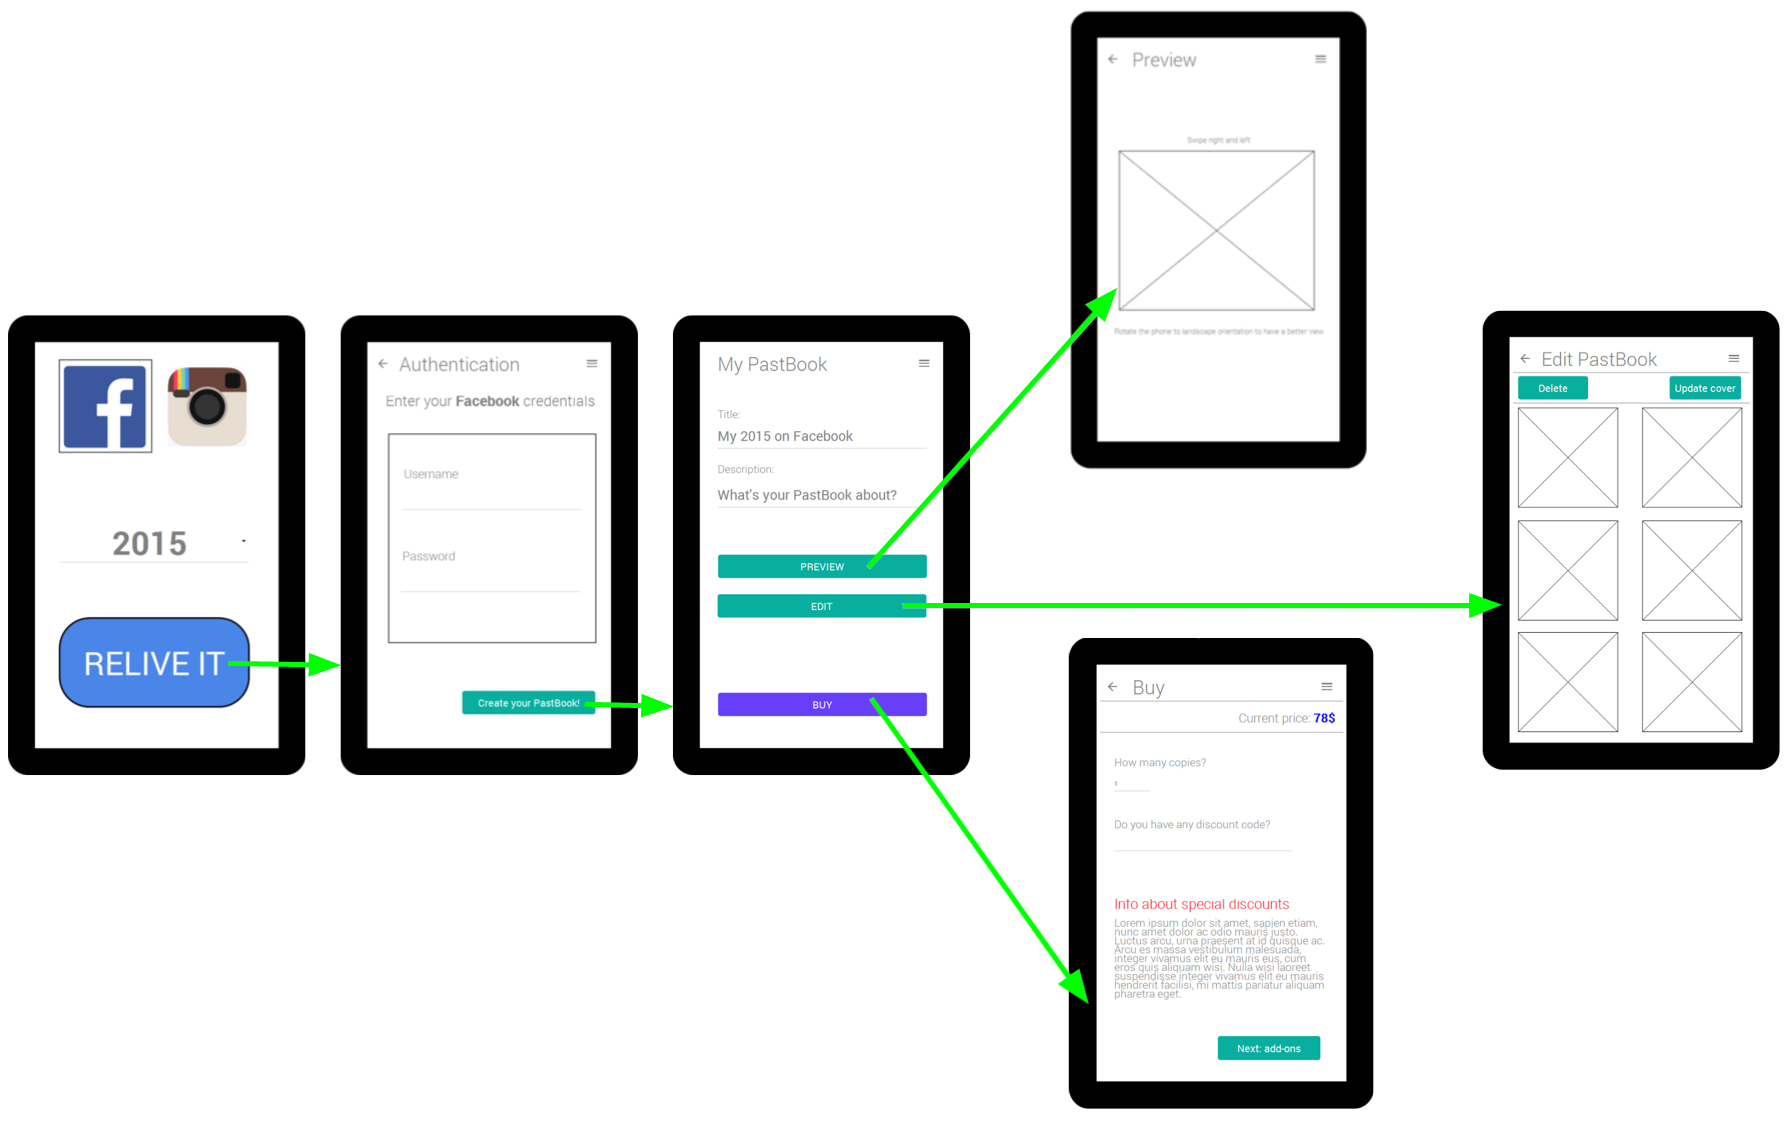
\includegraphics[width=0.95\textwidth]{capitolo_3/immagini/wireframe.png}
			\end{figure}
		\end{frame}
	\subsection{Sviluppo di My Year Photo Book}
		\begin{frame}{Implementazione dell'applicazione}
			\begin{minipage}{0.49\textwidth}
				\begin{minipage}{0.32\textwidth}
					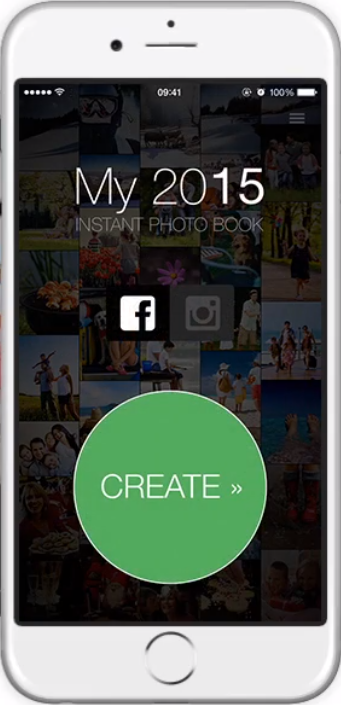
\includegraphics[width=1.0\textwidth]{capitolo_3/immagini/schermata_principale.png}
				\end{minipage}
				\begin{minipage}{0.32\textwidth}
					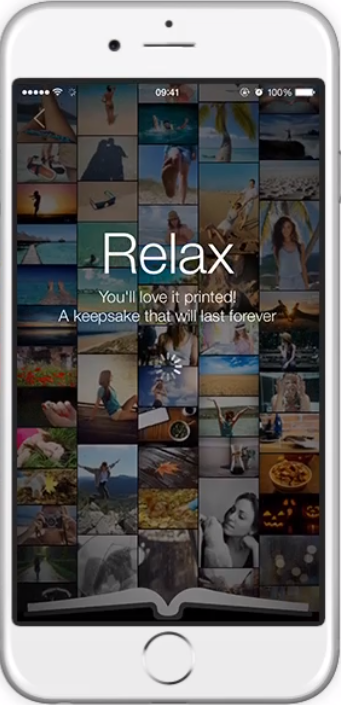
\includegraphics[width=1.0\textwidth]{capitolo_3/immagini/schermata_di_intrattenimento.png}
				\end{minipage}
				\begin{minipage}{0.32\textwidth}
					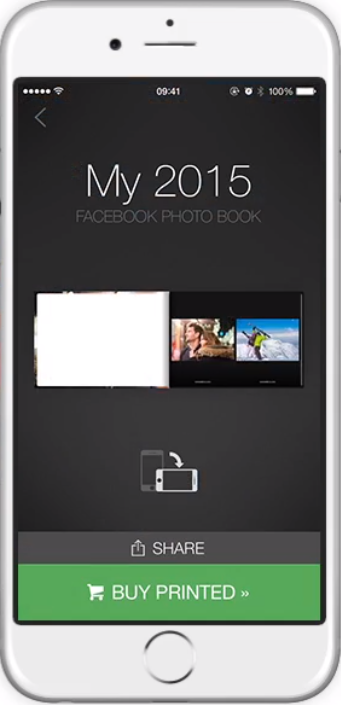
\includegraphics[width=1.0\textwidth]{capitolo_3/immagini/schermata_di_visualizzazione.png}
				\end{minipage}
			\end{minipage}
			\begin{minipage}{0.49\textwidth}
				\begin{itemize}
					\item Pattern architetturale MVC
					\item Componenti riutilizzabili
					\item \emph{Checkout} tramite Stripe
					\item \emph{Photo Book} “sfogliabile”
				\end{itemize}
			\end{minipage}\par
			\begin{block}{Schermata di intrattenimento}
				\begin{itemize}
					\item Uso delle funzioni del \emph{Launcher} (\emph{callback} e \emph{play/pause})
					\item Uso del componente \emph{gallery}
					\item Ottimizzazione delle prestazioni
				\end{itemize}
			\end{block}
		\end{frame}
